% Preamble
\documentclass[11pt]{article}
\usepackage{braket}
\usepackage{graphicx}
\usepackage[margin=1in]{geometry}

\usepackage{makeidx}  % allows for indexgeneration
\usepackage{ifpdf}
\usepackage{url}


\title{Elementary Cellular Automata as an Error Minimized Hash}
\date{November 2024}
\author{Daniel McKinley}

% Document
\begin{document}

\maketitle

\section{Introduction}

Elementary cellular automata (ECA) are 8 bit extensions of 4 bit logic gate truth tables, done linearly in parallel. \cite{Wolfram}
Here a subset of 8 of the 256 ECA rules are explored as a non-cryptographic hash function. It utilizes an error-minimization function on 4x4 binary grids; this parallels several discrete transforms, the Fast Fourier Transform (FFT) and Fast Walsh-Hadamard Transform. General algorithm, specific ECA rules, and aggregate properties are discussed. It is implemented in Java at \cite{mygit} along with more frames of the algorithm images. \\
\section{Main Algorithm}

\begin{center}
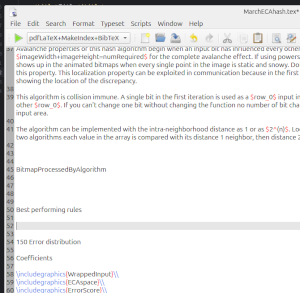
\includegraphics{testScreenshot}\\
Original Image\\
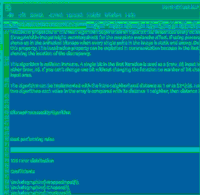
\includegraphics{processedDepth3}\\
Frame 3\\

\includegraphics{processedDepth6}\\
Frame 6\\
\end{center}

\begin{center}
There are $2^{16}=65536$ binary 4x4 arrays\\
 Where there are $2^4$ possible $row_0$ neighborhoods for a given ECA rule\\
 Each of these 16 input-ECAoutput arrays are scored by\\
\[  \sum_{r=0}^{3} \sum_{c=0}^{3} 2^r ( compressionAttempt_{r c} \oplus original_{r c}) \]\\
 The value of the neighborhoods of the minimum and maximum of these 16 sums are noted as the codeword of the original binary matrix  \\
\end{center}
The algorithm works on $2^n*2^n$ square matrices,2x2, 4x4, 8x8. The rest of this paper will refer to size 4x4. For all $2^(16)=655536$ possibilities of a 4x4 binary array, create a column-wrapped 4x4 array, use row 0 as the binary of all possible $2^4=16$ input neighborhoods; calculate the remaining three rows for all 16 possible input values using a standard log3 8 bit Wolfram code. For each of all these 16 possible inputs, score the 4x4 array with a weighted sum of discrepancies between this codeword-produced output and the original 4x4 matrix Input[][]. The lowest and highest scoring neighborhood are then two length-four codewords for a possible neighborhood of size 4x4. The algorithm's solutions for all neighborhoods of a certain size become a hexadecimal Wolfram code for a small QR code.  \\
\begin{center}
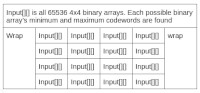
\includegraphics{inputGrid}\\
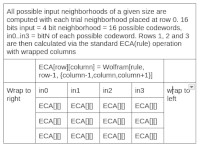
\includegraphics{ecaGrid}\\
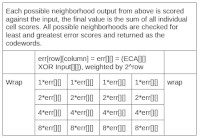
\includegraphics{errorGrid}\\
\end{center}

For every row,column location in input, that value's neighborhood is 4x4 (row,column)..((row+4),(column+4)). Every location is part of 16 neighborhoods. Transform the input so that each location is the minimizing and maximizing codewords of the ECA rule subset described later. If the input is depth 0, these codewords are depth 1. Depth 2 is the same process with the 4x4 neighborhoods' constituent rows and columns spaced out $2^{depth-1}$. Depth 1 is neighbors, depth 2 is two away, depth 3 is 4 away. This comparing of neighbors of powers of 2 is the same arrow chart as the FFT and Fast Walsh Transform, with reminimizations at every level of recursion. These exponential neighborhood expansions guarantee the avalanche property in $log_2(size)$ time.

This algorithm can both minimize the errorScore in a lossy compression, and maximize the errorScore. There are dual min-max versions of most variables in the implementation.\\

There are 8 [0,15,51,85,170,204,240,255] of the 256 8 bit ECA truth tables that display the properties of unique codewords for any given input and perfectly even distribution of codewords. 0 and 255 are included because in the 4 rows of the output matrix, 1 is neighborhood input and 3 are output, and still produce an errorScore. This subset works with both errorScore minimization and errorScore maximization. These two min max 8-tuples are implemented as a cryptographic hash.\\

A single rule of the positive 8-tuple of the above is a lossy compression algorithm with an error rate of 3/8. In a rectangular bitmap, the overlapping codeword, 16 4x4 neighbors that influence it, for all 8 of the rules in the subset together make a weighted vote on the inverse of the algorithm. 97 percent of bits were successfully recovered. Each codeword in the array produces a 4x4 ECA output that is its best guess about the information given to it. Each cell's 4x4 output overlaps with 4 of its neighbors. Each cell of each cell's output is weighted by its relative row and added to its location's tally of votes. At the end if the sum of the votes is positive then it becomes 0, if it is negative it becomes 1.

Codeword addition is each codeword's 4x4 ECA output is linearly added to another codeword and then the combination is itself reminimized. In constructing the addition tables for codewords, the result was a table that is exactly the logical operation row AND column. The Hadamard matrix can be constructed using this operation by summing the ones in (row AND column) taking it mod 2 for the boolean Hadamard matrix. Experimentally, in the inverse phase the binary Hadamard value of the codeword was substituted for the codeword's 4x4 ECA output. The result had roughly the same 97% decompression rate as the the first way. Each tuple rule's entire codeword output set was seperately processed as a weighted voting neighborhood without the overlap of the algorithm's main implementation. The result was 164/256 positively correlated Hadamard value to vote value. Each cell of each rule's Wolfram code does better than one half, then overlaps with 15 others al doing better than a 1/2.

Avalanche properties of this hash algorithm begin when an input bit has influenced every other input bit. If using sequential hashes, you need $imageWidth+imageHeight=numRequired$ for the complete avalanche effect. If using powers of two the avalanche effect begins at $log_2 (width) + log_2 (height)$. This property shows up in the animated bitmaps when every single point in the image is static and snowy. Doing fewer iterations than the avalanche's diffusion threshold but more than zero limits this property. This localization property can be exploited in communication because in the first few iterations the data is irreversible enough to be imperfectly unencryptable while showing the location of the discrepancy.\\

This algorithm has minimal collision resistance. The initial conversion from 4 hexadecimal places to 1 hexadecimal place mean every output 0-15 has 4096 other neighborhoods that produce the same thing. A general method of producing these collisions on command is under investigation. In certain image processing applications this property may be desireable, as images that are close but not quite hash closely as well.\\

The weight in the errorScore sum can be $2^{row}$ or $2^{column}$, both produce the same set of 8 tuples with the unique solution property, though other ECA rule's properties don't necessarily carry over.\\

The size of the input array can be easily be any power of 2 squared. Calculation of Wolfram code lengths of $2^{16}$ are acceptable, lengths of $2^{64}$ are in principle doable but not practical. However at size 8 there are $2^8=256$ possible codewords which grow exponentially but not doubly exponentially. The 8 tuple's uniqueness and distribution properties may apply at size 8 squared, it may not; it is only completely tested for size 4. Running statistics on random samples of size 8 have not been done yet.\\

Other rules\\

150 Error distribution\\

\bibliographystyle{plain}
\bibliography{HashBib.bib}

\end{document}